\documentclass[12pt, landscape]{article}
\usepackage[scaled=0.92]{helvet}
\usepackage{multicol}
\usepackage{calc}
\usepackage{ifthen}
\usepackage[landscape]{geometry}
%\usepackage{hyperref}

\usepackage{newtxtext} 

%for strikeout
\usepackage{ulem}

%For editing parbox
\usepackage[table]{xcolor}
%For editing itemise margins, reduce iterm separaion and list separation
\usepackage{enumitem}
% For math
\usepackage{amsmath,amsthm,amsfonts,amssymb}

%For pictures / figures
\usepackage{color,graphicx,overpic}
\graphicspath{ {./images/} }

%\usepackage{newtxtext} 
%\usepackage{amssymb}
%\usepackage[table]{xcolor}
%\usepackage{vwcol}
%\usepackage{tikz}
%\usepackage{wrapfig}
%\usepackage{makecell}

\pdfinfo{
  /Title (IS2238.pdf)
  /Creator (Ger Teck)
  /Author (Ger Teck)
  /Subject ()
  /Keywords (tex)}

%% Margins for PAPER

% This sets page margins to .5 inch if using letter paper, and to 1cm
% if using A4 paper. (This probably isn't strictly necessary.)
% If using another size paper, use default 1cm margins.
\ifthenelse{\lengthtest { \paperwidth = 11in}}
	{ \geometry{top=.5in,left=.5in,right=.5in,bottom=.5in} }
	{\ifthenelse{ \lengthtest{ \paperwidth = 297mm}}
		{\geometry{top=1cm,left=1cm,right=1cm,bottom=1cm} }
		{\geometry{top=1cm,left=1cm,right=1cm,bottom=1cm} }
	}

% Turn off header and footer
\pagestyle{empty}

% for tight centres (less spacing)
\newenvironment{tightcenter}{%
  \setlength\topsep{0pt}
  \setlength\parskip{0pt}
  \begin{center}
}{%
  \end{center}
}

% Redefine section commands to use less space
\makeatletter
\renewcommand{\section}{\@startsection{section}{1}{0mm}%
                                {-1ex plus -.5ex minus -.2ex}%
                                {0.5ex plus .2ex}%x
                                {\normalfont\large\bfseries}}
\renewcommand{\subsection}{\@startsection{subsection}{2}{0mm}%
                                {-1explus -.5ex minus -.2ex}%
                                {0.5ex plus .2ex}%
                                {\normalfont\normalsize\bfseries}}
\renewcommand{\subsubsection}{\@startsection{subsubsection}{3}{0mm}%
                                {-1ex plus -.5ex minus -.2ex}%
                                {1ex plus .2ex}%
                                {\normalfont\small\bfseries}}
% change font
%\renewcommand{\familydefault}{\sfdefault}
%\renewcommand\rmdefault{\sfdefault}
\makeatother

% Define BibTeX command
\def\BibTeX{{\rm B\kern-.05em{\sc i\kern-.025em b}\kern-.08em
    T\kern-.1667em\lower.7ex\hbox{E}\kern-.125emX}}

% Don't print section numbers
\setcounter{secnumdepth}{0}

\setlength{\parindent}{0pt}
\setlength{\parskip}{0pt plus 0.5ex}

%% this changes all items (enumerate and itemize, reduce margins)
\setlength{\leftmargini}{0.5cm}
\setlength{\leftmarginii}{0.5cm}
\setlist[itemize,1]{leftmargin=2mm,labelindent=1mm,labelsep=1mm, itemsep = 1mm}
\setlist[itemize,2]{leftmargin=4mm,labelindent=1mm,labelsep=1mm, itemsep = 1mm}
\itemsep = 2mm
%\setlist{nosep}

% -------------------------------------------------------------------------------

% START OF DOCUMENT HERE

\begin{document}
\raggedright
\footnotesize
\begin{multicols*}{3}

% multicol parameters
% These lengths are set only within the two main columns
\setlength{\columnseprule}{0pt}
\setlength{\premulticols}{1pt}
\setlength{\postmulticols}{1pt}
\setlength{\multicolsep}{2pt}
\setlength{\columnsep}{2pt}

%% DOCUMENT NAME HERE
\begin{center}
     \Large{\textbf{IS2238 Economics of IT \& AI}} \\
\end{center}

% TABLE PACKAGE 
 \begin{center}
    \fbox{%
        \parbox{0.8\linewidth}{\centering \textcolor{black}{
            \\ \normalsize{AY22/23 Sem 2}}
            \\ {\footnotesize github.com/gerteck}
        }%
    }
  \end{center}

\section{1. Overview of Economics of IT}

\begin{itemize}
	\item \textbf{IT/AI are changing our lives, businesses, and economy.} Economics can provide a lens through which we can better understand this new economy and phenomena in a more systematic manner.
	\item High speed change in today’s digital age. (Digital revolution). Cause of change is computer \& comunications, technology such as integreted circuits, data speed and laptop capacity which have increased by many times. $\rightarrow$ Increase in employee productivity.
	\item \textbf{Moore’s Law:} observation that the numer of transistors on a microchip doubles every 18-24 months (exponential growth). Advancement has slowed down since 2010s.
	\item \textbf{Why does IT matter for today's economy?}: IT capital investment by companies has grown steadily over the years from 1980s to 2010. Market capitalization has seen most large companies being tech related or heavily invested in IT.
	\item \textbf{Economics:} Allows for systematic understanding of new phenomena. This provides a lens through which we can better understand how things work, design clever solutions and create the conditions in which we can all flourish. We do this through economic theory, methods, analytical methods, empricial modelling.
	\item \textbf{Evaluating IT investment and its impact:} IT investments by firms do not necessarily lead to better outcomes nor better lives. Question has important policy and managerial implications. There are many variables to consider, such as obsolescence of old technologies, cost of learning, infrastructures, poor IT management, underutilization. Companies need to throughly understand the role and impact of IT on their business models and the exact use if implemented.
	\item \textbf{IT Productivity Paradox}: Economist Robert Solow: a Nobel Prize laureate, famously said in 1987, “You can see the computer age everywhere but in the productivity statistics”. It was largely resolved by an economics analysis done by MIT professor Erik Brynjolfsson and his colleagues in in the mid-1990s. Cobb–Douglas production function.
\end{itemize}

\subsection{Cobb-Douglas Production Function} 
models the relationship between production output and production inputs (factors).
\centerline{$Y = AL^\beta K^\alpha$}
\\ Y: Total Production, L: Labor Input,
\\ K: Capital Input, A: Total Factor Productivity,
\\ $\alpha$ and $\beta$: output elasticities of capital and labour.
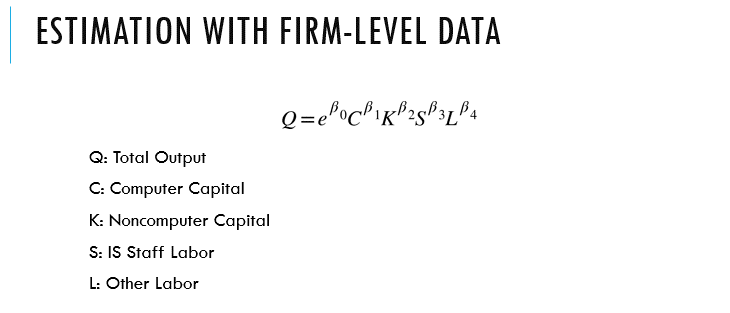
\includegraphics[width=\linewidth]{firmLevelData}

~\\

\textbf{Insights:} Brynjolfsson and Hitt (Management Science, 1996)
\begin{itemize}
\item An additional dollar of computer capital stock is associated with an increase in output of 81 cents per year on the margin An additional dollar spent was associated with a marginal increase in output of \$2.62
\end{itemize}

\vfill\null
\columnbreak

\section{2. Digital Economy and New IT}
\subsection{McKinsey View on 'New' IT}
\begin{itemize}
\item Numerous industries being `reimagined' through IT: To prevent a competitor from re-imagining your product as discontinued or re-imagining your company into liquidation, IT could well be an essential consideration in strategy formulation and execution, and a key area for investment.
\item `Old IT': Addressed labor automation, individual worker productivity, and non-human scale computing;
\item `New IT': Focus on digital products and services, team productivity, and business model transformation.
\item Benefits from old IT have reached a point of diminishing returns; new IT can be a source of competitive differentiation and dramatic wealth creation.
\item \textbf{Business Model Transformation} as a major use of IT, five major levers: Production and operations optimization, Eliminating intermediaries (bypassing middleman), New Monetization models (Amazon Web Services, SaaS etc.), Shaping customer preferences (leveraging big data), Transforming underserved markets (Long Tail phenomenon).
\end{itemize}

\subsection{Old Supply Chain Issues}
\begin{itemize}
\item Lack of Coordination between stages in the supply chain where objectives of different stages conflict or information moving between stages is distorted.
\item \textbf{Bullwhip Effect:} Fluctuations in order increases as they move up the supply chain from retailers to wholesalers to manufacturers to suppliers. Distorted demand information, where different stages have different estimates of what demand looks like, amplified variation in demand. Higher safety inventory usually required.
\item Information Processing Obstacles: Forecasting demand based on orders, not customer demand. Lack of information sharing. To overcome tradeoff, we trade responsiveness for cost and vice versa.
\end{itemize}

\subsection{Just-In-Time Production Methods}
\begin{itemize}
\item Tesla Motors has been using Just-In-Time (JIT) production methods to keep costs low since its founding in 2003. (JIT Benefits + Challenges) Tesla is experimenting with lean manufacturing principles in its production processes.
\item JIT is a production strategy that seeks to minimize waste and maximize efficiency by only producing what is needed, when it is needed. This approach requires close coordination between all parts of the production process, from suppliers to assembly line workers.
\item There are some chalenges associated with JIT, such as the need for tight coordination and the potential for disruptions to the production process. However, Tesla has shown that JIT can be an effective production strategy for a high-tech manufacturing company.
\end{itemize}

\subsection{Digital Economy}
\begin{itemize}
\item \textbf{A Digital Economy} takes advantage of the latest technology to digitalise processes and drive business growth. With digital economy, most of economic activities such as production, distribution, and consumption of goods and services are digitalized.
\item Digital technologies reduce the cost of storage, computation, and transmission of data. Therefore, digital economics explores how standard economic models change as certain costs fall substantially and perhaps approach zero.
\item \textbf{IT Capital Investment:} IT Capital Investment by companies has been increasing (in proportion and amount) over the years. IT automate many steps in business processes that were formerly performed manually. IT can enable new innovative business processes by collecting, processing, distributing information in a more efficient and effective way. (e.g., JIT, cross-docking) IT can transform the way the business works and drive new business models.
\end{itemize}
\textbf{Production and Economics of Production: Cost Curves}
\begin{itemize}
\item \textbf{Simple Economics of Production:}
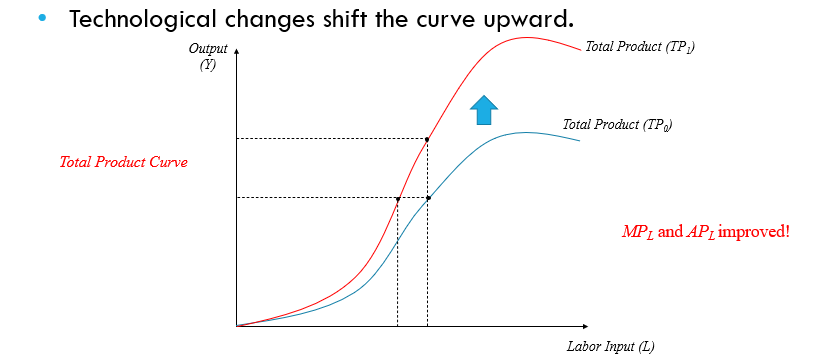
\includegraphics[width=0.7\linewidth]{technologicalChange}
\item \textbf{Economics of Digital Goods:} High fixed costs to produce the first unit, dominated by sunk cost: very high. Marginal production (reproduction) cost : very low. Hence, extensive economies of scale. Can be delivered via the Internet; little distribution cost.
\item DD and SS curve shifts as an impact of technological advances: Demand may shift leftward or rightward depending on the presence of substitutes or complements respectively. Supply increases generally as quality of product and cost of production changes due to technology.
\end{itemize}

\subsection{Disadvantages of Digital Economy}
\begin{itemize}
\item Digital divide: Generally refers to the gap between those who use or have access to telecommunications and information technologies including hardware, internet access, and literacy in using both effectively and those who do not.
\item Cybercrime and Privacy Breaches, Bad ideas spread quickly (e.g., fake news, racism, etc.), Pervasive Advertisement exposure (due to New business model), More monopolistic players (e.g., Google), Addictive nature of technology (Mental health and well-being concerns)
\end{itemize}

\textbf{Summary (of digital technology on businesses)}
\begin{itemize}
\item Digital technology enables economic activities such as production, distribution, and consumption of goods and services are conducted in a more efficient manner.
\item On top of that, digital innovation may lead to a fundamental change through a new economic rule, enhanced collaboration, and innovative business models.
\item However, some other challenges may also arise because of digital technologies
\end{itemize}

\vfill\null
\columnbreak

\section{3. Market Structure}
\begin{itemize}
\item \textbf{Market Power / Dominance} is the ability of a firm or group of firms within a market to profitably charge prices above the competitive level for a sustained period of time. Due to anti consumer and anti competitive issues, huge market power always reduces the economic wealth of society in many ways. (Sherman Antitrust Act US, M\&A regulation, price regulation.)
\item Surge in IT investment by firms from 1995: Internet and enterprise IT accelerated competition within traditional industries. Processes were digitalized through enterprise IT systems. Innovators dominate the market with better ways of doing things. Rivals recapture market shares by roling out further process innovations. Results in increased concentration, turbulence and performance spread.
\subsection{Market Structures (basic economics)}
\item \textbf{Perfect Competition}: Many buyers and sellers with small size, Homogeneous product (little differentiation), Perfect information for buyers and sellers, No transaction/switching costs in market, Free market entry and exit, Equal access to technologies, Company as a price taker. Equilibrium = Normal Profits
\item \textbf{Monopolistic Power}: A monopoly is a company that has "monopoly power" in the market for a particular good or service. The existence of a monopoly relies on the nature of its business. It is often one that displays one or several of the following qualities: Needs to operate under large economies of scale, Requires huge capital, No substitute, Government mandate ensuring its sole existence, Technological superiority and control resources. Disadvantages of a monopoly: Price fixing, declining product quality, loss of innovation, inflation.
\\ Arguments for a `Creative Monopoly': Some advantages of monopoly may include: Economies of scale, Stability of prices, R\&D spending.
\item \textbf{Oligopoly:}: An oligopoly consists of a select few companies that combined exert significant influence over a market or sector. Firms in this case either compete with another to collaborate together (collusion). They use their market influence to set the prices and in turn maximize their profits. Therefore, the consumers become the price takers. In an oligopoly, there are various barriers to entry in the market, and new firms find it difficult to establish themselves. Most countries have laws outlawing such anti-competitive behaviors. Think FAANG or MANGA.
\end{itemize}


\subsection{Porter's Five Forces Framework}
Five forces that determine the competitive intensity and therefore attractiveness of a market.
\begin{itemize}
\item A useful tool (i) to understand the attractiveness of an industry and (ii) to systematically analyze the external environment surrounding a firm. Overall industry attractiveness does not imply that every firm in the industry will return the same profitability. Competitive advantage of a firm is achieved by enhancing a firm’s ability to combat the 5 forces.
\item \textbf{Force 1: Bargining Power of Supplier}: Supplier power is high when there is domination of supply by a few companies. (Examples: Crude Oil Suppliers (OPEC)), product is unique or at least differentiated, has built up switching costs (Examples: Database (Oracle), MS Windows, Cell phone services), provides benefits through geographic proximity to its customers. ( Examples: Convenient stores), poses a definite threat to forward integrate into its customers’ business. (Examples: Movie studios that also own a chain of theatres).
\item \textbf{Force 2: Bargining Power of Buyer/Consumer}: Buyer’s bargaining power is high when it has large, concentrated buying power that enables it to gain volume discounts and/or special terms or services (Examples: organizational buyers like Wal-Mart, Costco, Safeway), what it is buying is standard or undifferentiated and there are multiple alternative sources, product is unimportant to the quality of the buyers’ products or services. (Examples: buyers of commodity type of products), has a strong potential to backward integration. (Examples: airline companies that also own aircraft maintenance and in-flight catering businesses).
\item \textbf{Force 3: Substitute Products or Services}: Substitutes: a product or service in another industry which can fulfill the same needs. Threat of substitute products or services is high when  Relative price performance of substitutes is high, Switching cost to new products is low, Buyer propensity to substitutes is large.
\item \textbf{Force 4: Threat of Potential New Entrants}: The threat of new entrants is high when it is easy for new competitors to enter a market, low when there are significant entry barriers to entering a market. Common sources of the entry barrier include: Regulation, Patents and proprietary knowledge, Economies of scale: Newcomer’s cost per product is higher, Capital requirement, Difficulty in brand switching, Difficulty in accessing distribution channel.
\item \textbf{Force 5: Rivalry among Existing Competitors}: Intra-industry rivalry is intense when Competitors are numerous or roughly equal in size and power, Industry growth is slow, precipitating fights for market share, and the product lacks differentiation or switching costs.
\end{itemize}

\subsection{Internet's Impact on Industries \& Forces}
\begin{itemize}
\item \textbf{Impact on Industries}: High Industry concentration, High Turbulence (the top-selling company one year may not dominate next year. Today’s \#10 company, for instance, might jump to \#1 the following year.) Large and Growing Performance Spread: Increasing spread in gross profit margin.
\item \textbf{Impact on Market Structures}: `Easier to become a monopoly in Digital Economy': Network Effects (“Winner takes all” phenomenon) (value of service depends on number of users), High switching cost, Economies of scale, High initial fixed cost and low marginal cost of production. Convergence of digital services (Blending of previously separate technologies, processes, and data to create new combinations of products, services, and experiences that reshape industry structures It is much easier to create new services by combining multiple services), AI \& Data analytics, Hard to regulate.
\item \textbf{Digital Business vs. Traditional Market:} Market definition is complicated by zero-pricing for the use of many digital platforms and the subsequent harvesting of consumer data. For many digital platforms, consumers forfeit their data (rather than money) in exchange for the services they receive (e.g., Google, YouTube, etc).
\item \textbf{Impact on Competitive Dynamic of each Force}:  Adds entry barriers to new entrances, enables foothold in rivalry among existing competitors, adds to switching cost reducing buyer power. (e.g. American Airlines (SABRE) Reservation system, Display bias, 80\% of reservation conducted on first page, Information over competitor, Co-host program with partner airlines bargining power, new business creation, enabled AA to expand busines scope into information business.)
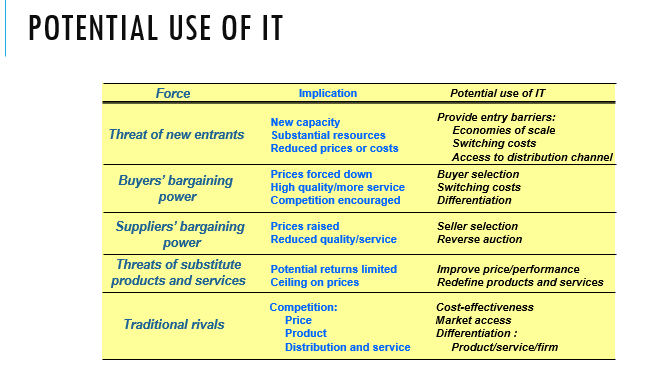
\includegraphics[width = 0.85\linewidth]{portersIT}
\textbf{Internet's Impact on Five Forces:}
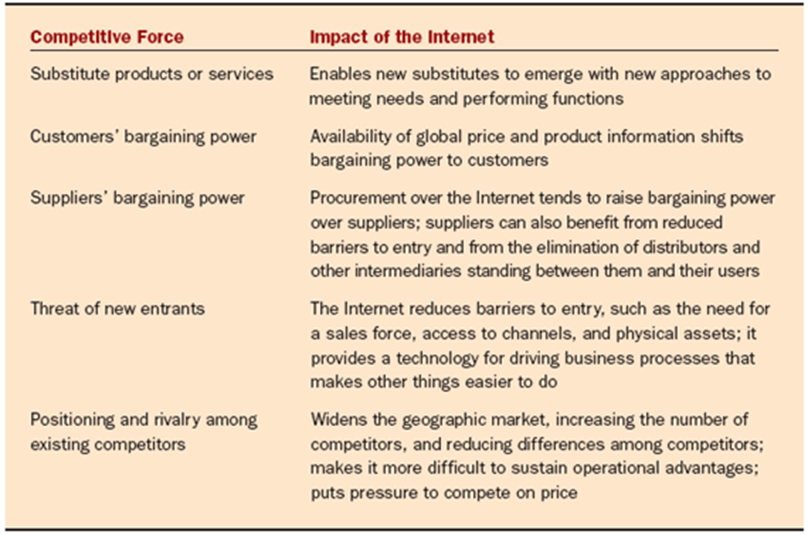
\includegraphics[width = \linewidth]{portersInternet}
\end{itemize}

\vfill\null
\columnbreak

\section{4. Pricing, Bundling and Subscription Model}


\vfill\null
\columnbreak

\section{5. Network Effects }



\vfill\null
\columnbreak

\section{6. Lock-in and Switching Costs}


\vfill\null
\columnbreak

\section{7. Free Riding and Contribution}


\vfill\null
\columnbreak

\section{8. Information Asymmetry / Transaction Cost Economics}


\vfill\null
\columnbreak

\section{9.  Search Cost \& Transaction Cost}


\vfill\null
\columnbreak

\section{10: Behavioral Economics}


\vfill\null
\columnbreak


\section{11: Economic Impacts of AI}



\vfill\null
\columnbreak


\section{12: Risks and Regulation of AI}










\end{multicols*}
\end{document}
